\documentclass{beamer}
\usetheme{ALUF}
\usepackage{animate}
\usepackage{algorithm}
\usepackage{algorithmic}
\usepackage{xcolor}
\usepackage{array}
\usepackage{media9}
\usepackage{tcolorbox}
% \usepackage{palatino}
% \usepackage[T1]{fontenc}
\usepackage{lmodern}
\usepackage{multimedia}
\usepackage{hyperref}
\usepackage[expert]{mathdesign}
\definecolor{lightblue}{rgb}{0.678, 0.847, 0.902}
\definecolor{graylight}{rgb}{0.8, 0.8, 0.8}
\definecolor{orange}{rgb}{1.0, 0.647, 0.0}
\definecolor{green}{rgb}{0.0, 1.0, 0.0}
\definecolor{red}{rgb}{1.0, 0.0, 0.0}
\newcommand{\highlightText}[1]{%
    \tikz[baseline]{%
        \node[fill=yellow!30,inner sep=2pt,blur shadow={shadow blur steps=5}] {#1};%
    }%
}
\usepackage[expert]{mathdesign}
\usepackage[protrusion=true,expansion=true,tracking=true,kerning=true]

\usepackage{tikz}

\usecolortheme{seahorse}
\setbeamertemplate{navigation symbols}{}
\setbeamertemplate{footline}[frame number]
\usepackage[sfdefault]{roboto}
\usepackage{fontawesome5}

\title{Randomised Algorithms}
\subtitle{Sometimes Randomness is faster}
\author{Mohtassim Masud [2105153]\\ Ahnaf Akib Tanim [2105154] \\Md.Shahjalal Rumman [2105165]}
\date{\today}
\institute{Department of CSE\\Bangladesh University of Engineering and Technology}

\begin{document}
\begin{frame}[plain,t]
    \hspace*{-1cm} % Shift the box to the left
    \parbox{\textwidth}{
        \titlepage
    }
\end{frame}

\begin{frame}% [plain,t]
	\frametitle{Outline}
\tableofcontents
\end{frame}

%=============================================================================================

%masud starts

\begin{frame}
    \frametitle{What is a Randomized Algorithm?}
    \textbf{Before diving into the definition...} \pause
    \vspace{0.5cm}
    \begin{block}{Let’s Begin with a Story!}
        Instead of starting with formalities, let's explore how randomness is applied in real-life scenarios: \pause
        \begin{itemize}
            \item How does \textbf{NASA} allocate critical tasks for its Mars Rovers fairly? \pause
            \item How does \textbf{Google} ensure the security of cryptocurrency transactions? \pause
        \end{itemize}
    \end{block}
    \vspace{0.8cm}
    \textbf{\textit{Let’s take a look at these examples to uncover the power of randomness!}}
\end{frame}

\section{Introduction}
\begin{frame}
    \frametitle{Randomness in NASA's Mars Rover}
    \textbf{Hardware Random Number Generator} \\
    \pause
    \begin{itemize}
        \item NASA announced a hardware random number generator for the Mars Rover. \pause
        \item Its purpose? To enhance decision-making by introducing randomness. \pause
        \item But randomness also introduces \textbf{possibilities of error}. \\
        \vspace{0.5cm}
        \centering
        \includegraphics[width=0.5\textwidth]{beamer-themes-master/ALUF/mars.jpeg} % Replace with an actual image
    \end{itemize}
\end{frame}
\begin{frame}
    \frametitle{Is Error-Free Randomness Possible?}
    \textbf{Uncertainty in the Physical World:} \\
    \pause
    \begin{itemize}
        \item In reality, \textbf{nothing is ever certain}. \pause
        \item Example: \textit{Radioactive contaminants in chips release alpha particles...} \pause
            \begin{itemize}
                \item Alpha particles flip memory bits unexpectedly. \pause
            \end{itemize}
        \item Cosmic rays cause \textbf{soft errors}—another unpredictable factor.
    \end{itemize}
    \vspace{0.5cm}
\end{frame}

\begin{frame}
	\frametitle{Notation}
	\begin{definition}[Randomized Algorithms]
		A randomized algorithm is an
            algorithm that incorporates randomness
            as part of its operation.

	\end{definition}
\end{frame}
% Slide for Deterministic Algorithms
\begin{frame}{Deterministic Algorithms}
% \hspace*{-5cm} % Shift the content to the left
\setbeamercovered{dynamic}

\begin{table}[]
    \centering
    \resizebox{1\textwidth}{!}{
    \begin{tabular}{l|l}
        
        \textbf{Aspect}            & \textbf{Deterministic Algorithm}                          \\ \hline\hline
       \onslide<2-> \textbf{Definition}        & Predefined set of rules, no randomness                   \\ \hline
       \onslide<3-> \textbf{Objective}         & Exact solutions with good worst-case behavior            \\ \hline
        \onslide<4->\textbf{Complexity}        & Often more complex with nuanced correctness proofs       \\ \hline
        \onslide<5->\textbf{Performance}       & Good in worst-case scenarios                             \\ \hline
        \onslide<6->\textbf{Error Tolerance}   & Guaranteed correctness                                   \\ 
    \end{tabular}
    }
    \caption{Characteristics of Deterministic Algorithms}
\end{table}
\end{frame}

% Slide for Randomized Algorithms
\begin{frame}{Randomized Algorithms}
\setbeamercovered{dynamic}
\begin{table}[]
    \centering
    \resizebox{1\textwidth}{!}{
    \begin{tabular}{l||l}
        \textbf{Aspect}            & \textbf{Randomized Algorithm}                            \\ \hline\hline
        \textbf{Definition}        & Incorporates randomness in its operation               \\ \hline
        \textbf{Objective}         & High probability of close-to-correct solutions         \\ \hline
        \textbf{Complexity}        & Simpler and denser analyses                            \\ \hline
        \textbf{Performance}       & Optimized for good average-case performance            \\ \hline
        \textbf{Error Tolerance}   & Small probability of error, adjustable by repetitions \\
    \end{tabular}
    }
    \caption{Characteristics of Randomized Algorithms}
\end{table}
\end{frame}
%%%%masud ends here
\section{Classic Quicksort and its Optimization}
\subsection{Quicksort}
\setbeamercovered{dynamic}
\begin{frame}{Pivot Sort!!}
    \textbf{\textcolor{blue}{Divide and Conquer:}} 
    \onslide<2->
    \begin{itemize}
        % \item Recursively partitions the array into smaller subarrays.
        \item Recursive partitions
        % \item Independently sorts each partition.
        \item Independent sorts
    \end{itemize}

    \vspace{0.5cm}
     \onslide<3->
    \textbf{\textcolor{red}{Time Complexity:}}
    \onslide<4->
    \begin{itemize}
    \onslide<5->
        \item \textcolor{violet}{Best/Average Case:} \( O(n\log n) \) (Balanced splits)
        \onslide<6->
        \item \textcolor{purple}{Worst Case:} \( O(n^2) \) (Highly unbalanced splits)
    \end{itemize}

    \vspace{0.5cm}
    \onslide<7->
    \begin{block}{\textbf{\textcolor{magenta}{Key Insight}}}
        \begin{center}
            % QuickSort’s efficiency depends heavily on how the pivot divides the array. 
            Pivot choice impacts efficiency.\\
            % \textbf{What happens if the pivot leads to poor splits?} 
            \textbf{\textcolor{cyan}{Poor Splits=?}} 
        \end{center}
    \end{block}
\end{frame}
\setbeamercovered{dynamic}
\subsection{The Algorithm}
\begin{frame}{QuickSort Algorithm}
    \begin{columns}
        \column{0.5\textwidth}
        \begin{exampleblock}{Algorithm QuickSort (Divide and Conquer)}
            \small
            \begin{algorithmic}[1]
                \STATE \textbf{Input:} Array \( A \), indices \( low, high \)
                \STATE \textbf{Output:} Sorted Array
                \IF{\( low < high \)}
                    \STATE \( pivot \gets \textcolor{}{\textbf{Partition}}(A, low, high) \)
                    \STATE QuickSort(A, low, pivot - 1)
                    \STATE QuickSort(A, pivot + 1, high)
                \ENDIF
            \end{algorithmic}
        \end{exampleblock}
         \onslide<2->
        \column{0.5\textwidth}
        \begin{exampleblock}{Algorithm Partition (Pivot Selection)}
            \small
            \begin{algorithmic}[1]
                \STATE \textbf{Input:} Array \( A \), indices \( low, high \)
                \STATE \textbf{Output:} Pivot index
                \STATE \( pivot \gets \textcolor{}{A[high]} \)
                \STATE \( i \gets low - 1 \)
                \FOR{\( j = low \) \textbf{to} \( high - 1 \)}
                    \IF{\( A[j] \leq pivot \)}
                        \STATE \( i \gets i + 1 \)
                        \STATE \textcolor{}{Swap \( A[i], A[j] \)}
                    \ENDIF
                \ENDFOR
                \STATE \textcolor{}{Swap \( A[i+1], A[high] \)}
                \RETURN \( i + 1 \)
            \end{algorithmic}
        \end{exampleblock}
    \end{columns}
    
    \end{frame}

%%%%%%%%%hereeeee
\begin{frame}[t]{Example Simulation}
\onslide<2->
    \begin{columns}[T]
        \begin{column}{0.95\textwidth}
            \begin{exampleblock}{}
                \scriptsize
                \begin{tabular}{l}
                    \textcolor{red}{pivot} $\gets A[high]$ \\[0.1cm]
                     \highlightText{\textcolor{orange}{i} $\gets$$low - 1$} \\[0.2cm]
                     \highlightText{\textbf{for} $\textcolor{orange}{j} =$$low$} \textbf{to} $high - 1$ \textbf{do} \\[0.1cm]
                    \hspace{0.4cm}\textbf{if} $A[j] \leq \textcolor{red}{pivot}$ \textbf{then} \\[0.2cm]
                    \hspace{1cm}\textcolor{orange}{i} $\gets$ \textcolor{orange}{i} + 1 \\[0.1cm]
                    \hspace{1cm}\textcolor{green}{Swap}(A[i], A[j]) \\[0.1cm]
                    \hspace{0.4cm}\textbf{end if} \\[0.1cm]
                    \textbf{end for} \\[0.2cm]
                    \textcolor{green}{Swap}(A[i+1], A[high]) \\[0.1cm]
                    \textbf{return} \textcolor{orange}{i + 1}
                \end{tabular}
            \end{exampleblock}
        \end{column}
    \end{columns}
    \onslide<1->
    \vspace{0.1cm}
    \begin{center}
    \small
    \textbf{Pivot}: \tikz\draw[fill=lightblue, minimum width=0.4cm, minimum height=0.4cm] (0,0) rectangle (0.2,0.2);
    \textbf{i}: \tikz\draw[fill=orange, minimum width=0.4cm, minimum height=0.4cm] (0,0) rectangle (0.2,0.2);
    \textbf{j}: \tikz\draw[fill=green, minimum width=0.4cm, minimum height=0.4cm] (0,0) rectangle (0.2,0.2);
    \textbf{Swap}: \tikz\draw[fill=black, minimum width=0.4cm, minimum height=0.4cm] (0,0) rectangle (0.2,0.2);
    \end{center}
    
    \vspace{-0.2cm}
    \hspace{-0.2cm}
    \begin{tikzpicture}[transform canvas={scale=0.9}]
        \node[draw, fill=orange, minimum width=0.9cm, minimum height=0.9cm] (a1) at (1,0) {i=-1};
        \node[draw, fill=green, minimum width=0.9cm, minimum height=0.9cm] (a2) at (3,0) {5};
        \node[draw, fill=graylight, minimum width=0.9cm, minimum height=0.9cm] (a3) at (5,0) {4};
        \node[draw, fill=graylight, minimum width=0.9cm, minimum height=0.9cm] (a4) at (7,0) {2};
        \node[draw, fill=graylight, minimum width=0.9cm, minimum height=0.9cm] (a5) at (9,0) {1};
        \node[draw, fill=lightblue, minimum width=0.9cm, minimum height=0.9cm] (a6) at (11,0) {3};
    \end{tikzpicture}
    
    \vspace{0.3cm}
\end{frame}
\begin{frame}[t]{Example Simulation}
\onslide<2->
    \begin{columns}[T]
        \begin{column}{0.95\textwidth}
            \begin{exampleblock}{}
                \scriptsize
                \begin{tabular}{l}
                    \textcolor{red}{pivot} $\gets A[high]$ \\[0.1cm]
                    \textcolor{orange}{i} $\gets low - 1$ \\[0.1cm]
                    \textbf{for} $\textcolor{orange}{j} = low$ \textbf{to} $high - 1$ \textbf{do} \\[0.1cm]
                    \hspace{0.4cm}\textbf{if} $A[j] \leq \textcolor{red}{pivot}$ \textbf{then} \\[0.1cm]
                    \hspace{1cm}\textcolor{orange}{i} $\gets$ \textcolor{orange}{i} + 1 \\[0.1cm]
                    \hspace{1cm}\textcolor{green}{Swap}(A[i], A[j]) \\[0.2cm]
                   \hspace{0.4cm}\textbf{end if} \colorbox{lightblue}{\textbf{\textcolor{red}{i not getting updated}}} \\[0.1cm]
                    \textbf{end for} \\[0.1cm]
                    \textcolor{green}{Swap}(A[i+1], A[high]) \\[0.1cm]
                    \textbf{return} \textcolor{orange}{i + 1}
                \end{tabular}
            \end{exampleblock}
        \end{column}
    \end{columns}
    \onslide<1->
    \vspace{0.2cm}  % Reduced spacing here
    
    \begin{center}
    \small
    \textbf{Pivot}: \tikz\draw[fill=lightblue, minimum width=0.4cm, minimum height=0.4cm] (0,0) rectangle (0.2,0.2);
    \textbf{i}: \tikz\draw[fill=orange, minimum width=0.4cm, minimum height=0.4cm] (0,0) rectangle (0.2,0.2);
    \textbf{j}: \tikz\draw[fill=green, minimum width=0.4cm, minimum height=0.4cm] (0,0) rectangle (0.2,0.2);
    \textbf{Swap}: \tikz\draw[fill=black, minimum width=0.4cm, minimum height=0.4cm] (0,0) rectangle (0.2,0.2);
    \end{center}
    
    \vspace{-0.2cm}  % Added negative spacing to move TikZ picture up
        \hspace*{-0.5cm}
    \begin{tikzpicture}[transform canvas={scale=0.9}]
        \node[draw, fill=orange, minimum width=0.9cm, minimum height=0.9cm] (a1) at (1,0) {i=-1};
        \node[draw, fill=graylight, minimum width=0.9cm, minimum height=0.9cm] (a2) at (3,0) {5};
        \node[draw, fill=green, minimum width=0.9cm, minimum height=0.9cm] (a3) at (5,0) {4};
        \node[draw, fill=graylight, minimum width=0.9cm, minimum height=0.9cm] (a4) at (7,0) {2};
        \node[draw, fill=graylight, minimum width=0.9cm, minimum height=0.9cm] (a5) at (9,0) {1};
        \node[draw, fill=lightblue, minimum width=0.9cm, minimum height=0.9cm] (a6) at (11,0) {3};
    \end{tikzpicture}
        \hspace*{-2cm}
    \vspace{0.3cm}  % Added spacing at the bottom to prevent touching frame border
\end{frame}
%%%%h2222
\begin{frame}[t]{Example Simulation}
\onslide<2->
    \begin{columns}[T]
        \begin{column}{0.95\textwidth}
            \begin{exampleblock}{}
                \scriptsize
                \begin{tabular}{l}
                    \hspace{0.5cm} \textcolor{red}{pivot} $\gets A[high]$ \\[0.1cm]
                    \hspace{0.5cm} \textcolor{orange}{i} $\gets low - 1$ \\[0.1cm]
                    \hspace{0.5cm} \textbf{for} $\textcolor{orange}{j} = low$ \textbf{to} $high - 1$ \textbf{do} \\[0.1cm]
                    \hspace{1cm} \textbf{if} $A[j] \leq \textcolor{red}{pivot}$ \textbf{then} \\[0.1cm]
                    \hspace{1.5cm} \tikz[baseline]{\node[anchor=base, draw=none, fill=lightgray, blur shadow={shadow blur steps=5}] {\Large \textcolor{orange}{i $\gets$ i + 1}};} \\[0.1cm]
                    \hspace{1.5cm} \tikz[baseline]{\node[anchor=base, draw=none, fill=lightgray, blur shadow={shadow blur steps=5}] {\textcolor{green}{Swap}(A[i], A[j]);};} \\[0.2cm]
                    \hspace{1cm} \textbf{end if} \\[0.1cm]
                    \hspace{0.5cm} \textbf{end for} \\[0.1cm]
                    \hspace{0.5cm} \textcolor{green}{Swap}(A[i+1], A[high]) \\[0.1cm]
                    \hspace{0.5cm} \textbf{return} \textcolor{orange}{i + 1}
                \end{tabular}
            \end{exampleblock}
        \end{column}
    \end{columns}
    \onslide<1->
    \vspace{0.1cm}

    \begin{center}
    \small
    \textbf{Pivot}: \tikz\draw[fill=lightblue, minimum width=0.4cm, minimum height=0.4cm] (0,0) rectangle (0.2,0.2);
    \textbf{i}: \tikz\draw[fill=orange, minimum width=0.4cm, minimum height=0.4cm] (0,0) rectangle (0.2,0.2);
    \textbf{j}: \tikz\draw[fill=green, minimum width=0.4cm, minimum height=0.4cm] (0,0) rectangle (0.2,0.2);
    \textbf{Swap}: \tikz\draw[fill=black, minimum width=0.4cm, minimum height=0.4cm] (0,0) rectangle (0.2,0.2);
    \end{center}

    \vspace{-0.2cm}
    \hspace*{-1.5cm}
    \begin{tikzpicture}[transform canvas={scale=0.9}]
        \node[draw, fill=orange, blur shadow={shadow blur steps=-1}, minimum width=1.2cm, minimum height=1.2cm] (a2) at (3,0) {5};
        \node[draw, fill=graylight, minimum width=1cm, minimum height=1cm] (a3) at (5,0) {4};
        \node[draw, fill=green, blur shadow={shadow blur steps=-1}, minimum width=1.2cm, minimum height=1.2cm] (a4) at (7,0) {2};
        \node[draw, fill=graylight, minimum width=0.9cm, minimum height=0.9cm] (a5) at (9,0) {1};
        \node[draw, fill=lightblue, minimum width=0.9cm, minimum height=0.9cm] (a6) at (11,0) {3};
        \draw[->, thick, bend left=45] (a2) to node[above, sloped, midway] {Swap} (a4);
    \end{tikzpicture}
    \hspace*{-2cm}
    \vspace{0.3cm}
\end{frame}
%%%%%h3333
\begin{frame}[t]{Example Simulation}
    \begin{columns}[T]
        \begin{column}{0.95\textwidth}
            \begin{exampleblock}{}
                \scriptsize
                \begin{tabular}{l}
                    \hspace{0.5cm} \textcolor{red}{pivot} $\gets A[high]$ \\[0.1cm]
                    \hspace{0.5cm} \textcolor{orange}{i} $\gets low - 1$ \\[0.1cm]
                    \hspace{0.5cm} \textbf{for} $\textcolor{orange}{j} = low$ \textbf{to} $high - 1$ \textbf{do} \\[0.1cm]
                    \hspace{1cm} \textbf{if} $A[j] \leq \textcolor{red}{pivot}$ \textbf{then} \\[0.1cm]
                    \hspace{1cm}\textcolor{orange}{i} $\gets$ \textcolor{orange}{i} + 1 \\[0.1cm]
                    \hspace{1cm}\textcolor{green}{Swap}(A[i], A[j]) \\[0.1cm]
                    \hspace{1cm} \textbf{end if} \\[0.1cm]
                    \hspace{0.5cm} \textbf{end for} \\[0.1cm]
                    \hspace{0.5cm} \textcolor{green}{Swap}(A[i+1], A[high]) \\[0.1cm]
                    \hspace{0.5cm} \textbf{return} \textcolor{orange}{i + 1}
                \end{tabular}
            \end{exampleblock}
        \end{column}
    \end{columns}
    \vspace{0.1cm}

    \begin{center}
    \small
    \textbf{Pivot}: \tikz\draw[fill=lightblue, minimum width=0.4cm, minimum height=0.4cm] (0,0) rectangle (0.2,0.2);
    \textbf{i}: \tikz\draw[fill=orange, minimum width=0.4cm, minimum height=0.4cm] (0,0) rectangle (0.2,0.2);
    \textbf{j}: \tikz\draw[fill=green, minimum width=0.4cm, minimum height=0.4cm] (0,0) rectangle (0.2,0.2);
    \textbf{Swap}: \tikz\draw[fill=black, minimum width=0.4cm, minimum height=0.4cm] (0,0) rectangle (0.2,0.2);
    \end{center}

    \vspace{-0.2cm}
    \hspace*{-1.5cm}
    \begin{tikzpicture}[transform canvas={scale=0.9}]
        \node[draw, fill=orange, blur shadow={shadow blur steps=-1}, minimum width=1.2cm, minimum height=1.2cm] (a2) at (3,0) {2};
        \node[draw, fill=graylight, minimum width=1cm, minimum height=1cm] (a3) at (5,0) {4};
        \node[draw, fill=green, blur shadow={shadow blur steps=-1}, minimum width=1.2cm, minimum height=1.2cm] (a4) at (7,0) {5};
        \node[draw, fill=graylight, minimum width=0.9cm, minimum height=0.9cm] (a5) at (9,0) {1};
        \node[draw, fill=lightblue, minimum width=0.9cm, minimum height=0.9cm] (a6) at (11,0) {3};
    \end{tikzpicture}
        \hspace*{-2cm}
    \vspace{0.2cm}
\end{frame}
\begin{frame}[t]{Example Simulation}
\onslide<2->
    \begin{columns}[T]
        \begin{column}{0.95\textwidth}
            \begin{exampleblock}{}
                \scriptsize
                \begin{tabular}{l}
                    \hspace{0.5cm} \textcolor{red}{pivot} $\gets A[high]$ \\[0.1cm]
                    \hspace{0.5cm} \textcolor{orange}{i} $\gets low - 1$ \\[0.1cm]
                    \hspace{0.5cm} \textbf{for} $\textcolor{orange}{j} = low$ \textbf{to} $high - 1$ \textbf{do} \\[0.1cm]
                    \hspace{1cm} \textbf{if} $A[j] \leq \textcolor{red}{pivot}$ \textbf{then} \\[0.1cm]
                    \hspace{1.5cm} \tikz[baseline]{\node[anchor=base, draw=none, fill=lightgray, blur shadow={shadow blur steps=5}] {\Large \textcolor{orange}{i $\gets$ i + 1}};} \\[0.1cm]
                    \hspace{1.5cm} \tikz[baseline]{\node[anchor=base, draw=none, fill=lightgray, blur shadow={shadow blur steps=5}] {\textcolor{green}{Swap}(A[i], A[j]);};} \\[0.2cm]
                    \hspace{1cm} \textbf{end if} \\[0.1cm]
                    \hspace{0.5cm} \textbf{end for} \\[0.1cm]
                    \hspace{0.5cm} \textcolor{green}{Swap}(A[i+1], A[high]) \\[0.1cm]
                    \hspace{0.5cm} \textbf{return} \textcolor{orange}{i + 1}
                \end{tabular}
            \end{exampleblock}
        \end{column}
    \end{columns}
    \onslide<1->
    \vspace{0.1cm}

    \begin{center}
    \small
    \textbf{Pivot}: \tikz\draw[fill=lightblue, minimum width=0.4cm, minimum height=0.4cm] (0,0) rectangle (0.2,0.2);
    \textbf{i}: \tikz\draw[fill=orange, minimum width=0.4cm, minimum height=0.4cm] (0,0) rectangle (0.2,0.2);
    \textbf{j}: \tikz\draw[fill=green, minimum width=0.4cm, minimum height=0.4cm] (0,0) rectangle (0.2,0.2);
    \textbf{Swap}: \tikz\draw[fill=black, minimum width=0.4cm, minimum height=0.4cm] (0,0) rectangle (0.2,0.2);
    \end{center}
    \vspace{-0.2cm}
    \hspace*{-1.5cm}
    \begin{tikzpicture}[transform canvas={scale=0.9}]
        \node[draw, fill=graylight, minimum width=0.9cm, minimum height=0.9cm] (a2) at (3,0) {2};
        \node[draw, fill=orange, minimum width=1.2cm, minimum height=1.2cm] (a3) at (5,0) {4};
        \node[draw, fill=graylight, minimum width=0.9cm, minimum height=0.9cm] (a4) at (7,0) {5};
        \node[draw, fill=green, blur shadow={shadow blur steps=-1},minimum width=1.2cm, minimum height=1.2cm] (a5) at (9,0) {1};
        \node[draw, fill=lightblue, minimum width=0.9cm, minimum height=0.9cm] (a6) at (11,0) {3};
        \draw[->, thick, bend left=45] (a3) to node[above, sloped, midway] {Swap} (a5);
    \end{tikzpicture}
  \hspace*{-2cm}  
    
    \vspace{0.3cm}
\end{frame}
%%%%%h444
\begin{frame}[t]{Example Simulation}
    \begin{columns}[T]
        \begin{column}{0.95\textwidth}
            \begin{exampleblock}{}
                \scriptsize
                \begin{tabular}{l}
                    \hspace{0.5cm} \textcolor{red}{pivot} $\gets A[high]$ \\[0.1cm]
                    \hspace{0.5cm} \textcolor{orange}{i} $\gets low - 1$ \\[0.1cm]
                    \hspace{0.5cm} \textbf{for} $\textcolor{orange}{j} = low$ \textbf{to} $high - 1$ \textbf{do} \\[0.1cm]
                    \hspace{1cm} \textbf{if} $A[j] \leq \textcolor{red}{pivot}$ \textbf{then} \\[0.1cm]
                    \hspace{1cm}\textcolor{orange}{i} $\gets$ \textcolor{orange}{i} + 1 \\[0.1cm]
                    \hspace{1cm}\textcolor{green}{Swap}(A[i], A[j]) \\[0.1cm]
                    \hspace{1cm} \textbf{end if} \\[0.1cm]
                    \hspace{0.5cm} \textbf{end for} \\[0.1cm]
                    \hspace{0.5cm} \textcolor{green}{Swap}(A[i+1], A[high]) \\[0.1cm]
                    \hspace{0.5cm} \textbf{return} \textcolor{orange}{i + 1}
                \end{tabular}
            \end{exampleblock}
        \end{column}
    \end{columns}
    \vspace{0.1cm}

    \begin{center}
    \small
    \textbf{Pivot}: \tikz\draw[fill=lightblue, minimum width=0.4cm, minimum height=0.4cm] (0,0) rectangle (0.2,0.2);
    \textbf{i}: \tikz\draw[fill=orange, minimum width=0.4cm, minimum height=0.4cm] (0,0) rectangle (0.2,0.2);
    \textbf{j}: \tikz\draw[fill=green, minimum width=0.4cm, minimum height=0.4cm] (0,0) rectangle (0.2,0.2);
    \textbf{Swap}: \tikz\draw[fill=black, minimum width=0.4cm, minimum height=0.4cm] (0,0) rectangle (0.2,0.2);
    \end{center}

    \vspace{-0.1cm}
\hspace*{-1.5cm}
% \hspace*{-2cm}
%     \vspace{0.3cm}
    \begin{tikzpicture}[transform canvas={scale=0.9}]
        \node[draw, fill=graylight, minimum width=0.9cm, minimum height=0.9cm] (a2) at (3,0) {2};
        \node[draw, fill=orange, minimum width=1.2cm, minimum height=1.2cm] (a3) at (5,0) {1};
        \node[draw, fill=graylight, minimum width=0.9cm, minimum height=0.9cm] (a4) at (7,0) {5};
        \node[draw, fill=graylight,minimum width=0.9cm, minimum height=0.9cm] (a5) at (9,0) {4};
        \node[draw, fill=green,blur shadow={shadow blur steps=-1}, minimum width=1.2cm, minimum height=1.2cm] (a6) at (11,0) {3};
    \end{tikzpicture}
    \hspace*{-2cm}
    \vspace{0.3cm}
\end{frame}
\begin{frame}[t]{Example Simulation}
\onslide<2->
    \begin{columns}[T]
        \begin{column}{0.95\textwidth}
            \begin{exampleblock}{}
                \scriptsize
                \begin{tabular}{l}
                    \hspace{0.5cm} \textcolor{red}{pivot} $\gets A[high]$ \\[0.1cm]
                    \hspace{0.5cm} \textcolor{orange}{i} $\gets low - 1$ \\[0.1cm]
                    \hspace{0.5cm} \textbf{for} $\textcolor{orange}{j} = low$ \textbf{to} $high - 1$ \textbf{do} \\[0.1cm]
                    \hspace{1cm} \textbf{if} $A[j] \leq \textcolor{red}{pivot}$ \textbf{then} \\[0.1cm]
                     \hspace{1.5cm} \tikz[baseline]{\node[anchor=base, draw=none, fill=lightgray, blur shadow={shadow blur steps=5}] {\Large \textcolor{orange}{i $\gets$ i + 1}};} \\[0.1cm]
                    \hspace{1.5cm} \tikz[baseline]{\node[anchor=base, draw=none, fill=lightgray, blur shadow={shadow blur steps=5}] {\textcolor{green}{Swap}(A[i], A[j]);};} \\[0.2cm]
                    \hspace{1cm} \textbf{end if} \\[0.1cm]
                    \hspace{0.5cm} \textbf{end for} \\[0.1cm]
                    \hspace{0.5cm} \textcolor{green}{Swap}(A[i+1], A[high]) \\[0.1cm]
                    \hspace{0.5cm} \textbf{return} \textcolor{orange}{i + 1}
                \end{tabular}
            \end{exampleblock}
        \end{column}
    \end{columns}
    \vspace{0.1cm}
\onslide<1->
    \begin{center}
    \small
    \textbf{Pivot}: \tikz\draw[fill=lightblue, minimum width=0.4cm, minimum height=0.4cm] (0,0) rectangle (0.2,0.2);
    \textbf{i}: \tikz\draw[fill=orange, minimum width=0.4cm, minimum height=0.4cm] (0,0) rectangle (0.2,0.2);
    \textbf{j}: \tikz\draw[fill=green, minimum width=0.4cm, minimum height=0.4cm] (0,0) rectangle (0.2,0.2);
    \textbf{Swap}: \tikz\draw[fill=black, minimum width=0.4cm, minimum height=0.4cm] (0,0) rectangle (0.2,0.2);
    \end{center}

    \vspace{-0.1cm}
\hspace*{-1.5cm}
% \hspace*{-2cm}
%     \vspace{0.3cm}
    \begin{tikzpicture}[transform canvas={scale=0.9}]
        \node[draw, fill=graylight, minimum width=0.9cm, minimum height=0.9cm] (a2) at (3,0) {2};
        \node[draw, fill=graylight, minimum width=0.9cm, minimum height=0.9cm] (a3) at (5,0) {1};
        \node[draw, fill=orange, minimum width=1.2cm, minimum height=1.2cm] (a4) at (7,0) {5};
        \node[draw, fill=graylight,minimum width=0.9cm, minimum height=0.9cm] (a5) at (9,0) {4};
        \node[draw, fill=green,blur shadow={shadow blur steps=-1}, minimum width=1.2cm, minimum height=1.2cm] (a6) at (11,0) {3};
         \draw[->, thick, bend left=45] (a4) to node[above, sloped, midway] {Swap} (a6);
    \end{tikzpicture}
    \hspace*{-2cm}
    \vspace{0.3cm}
\end{frame}
\begin{frame}[t]{Example Simulation}
    \begin{columns}[T]
        \begin{column}{0.95\textwidth}
            \begin{exampleblock}{}
                \scriptsize
                \begin{tabular}{l}
                    \hspace{0.5cm} \textcolor{red}{pivot} $\gets A[high]$ \\[0.1cm]
                    \hspace{0.5cm} \textcolor{orange}{i} $\gets low - 1$ \\[0.1cm]
                    \hspace{0.5cm} \textbf{for} $\textcolor{orange}{j} = low$ \textbf{to} $high - 1$ \textbf{do} \\[0.1cm]
                    \hspace{1cm} \textbf{if} $A[j] \leq \textcolor{red}{pivot}$ \textbf{then} \\[0.1cm]
                     \hspace{1cm}\textcolor{orange}{i} $\gets$ \textcolor{orange}{i} + 1 \\[0.1cm]
                    \hspace{1cm}\textcolor{green}{Swap}(A[i], A[j]) \\[0.1cm]
                    \hspace{1cm} \textbf{end if} \\[0.1cm]
                    \hspace{0.5cm} \textbf{end for} \\[0.1cm]
                    \hspace{0.5cm} \textcolor{green}{Swap}(A[i+1], A[high]) \\[0.1cm]
                    \hspace{0.5cm} \textbf{return} \textcolor{orange}{i + 1}
                \end{tabular}
            \end{exampleblock}
        \end{column}
    \end{columns}
    \vspace{0.1cm}

    \begin{center}
    \small
    \textbf{Pivot}: \tikz\draw[fill=lightblue, minimum width=0.4cm, minimum height=0.4cm] (0,0) rectangle (0.2,0.2);
    \textbf{i}: \tikz\draw[fill=orange, minimum width=0.4cm, minimum height=0.4cm] (0,0) rectangle (0.2,0.2);
    \textbf{j}: \tikz\draw[fill=green, minimum width=0.4cm, minimum height=0.4cm] (0,0) rectangle (0.2,0.2);
    \textbf{Swap}: \tikz\draw[fill=black, minimum width=0.4cm, minimum height=0.4cm] (0,0) rectangle (0.2,0.2);
    \end{center}

    \vspace{-0.1cm}
\hspace*{-1.5cm}
% \hspace*{-2cm}
%     \vspace{0.3cm}
    \begin{tikzpicture}[transform canvas={scale=0.9}]
        \node[draw, fill=graylight, minimum width=0.9cm, minimum height=0.9cm] (a2) at (3,0) {2};
        \node[draw, fill=graylight, minimum width=0.9cm, minimum height=0.9cm] (a3) at (5,0) {1};
        \node[draw, fill=graylight, minimum width=0.9cm, minimum height=0.9cm] (a4) at (7,0) {3};
        \node[draw, fill=graylight,minimum width=0.9cm, minimum height=0.9cm] (a5) at (9,0) {4};
        \node[draw, fill=lightblue, minimum width=1.2cm, minimum height=1.2cm] (a6) at (11,0) {5};
\node[above=0.2cm, text=red, font=\bfseries\Large] at (a6.north) {New Pivot};

    \end{tikzpicture}
    \hspace*{-2cm}
    \vspace{0.3cm}
\end{frame}
\begin{frame}[t]{Example Simulation}
\onslide<2->
    \begin{columns}[T]
        \begin{column}{0.55\textwidth}
            \begin{exampleblock}{QuickSort Partitioning}
                \scriptsize
                \begin{tabular}{l}
                    \hspace{0.5cm} \textcolor{red}{pivot} $\gets A[high]$ \\[0.1cm]
                    \hspace{0.5cm} \textcolor{orange}{i} $\gets low - 1$ \\[0.1cm]
                    \hspace{0.5cm} \textbf{for} $\textcolor{orange}{j} = low$ \textbf{to} $high - 1$ \textbf{do} \\[0.1cm]
                    \hspace{1cm} \textbf{if} $A[j] \leq \textcolor{red}{pivot}$ \textbf{then} \\[0.1cm]
                    \hspace{1cm} \textcolor{orange}{i} $\gets$ \textcolor{orange}{i} + 1 \\[0.1cm]
                    \hspace{1cm} \textcolor{green}{Swap}(A[i], A[j]) \\[0.1cm]
                    \hspace{1cm} \textbf{end if} \\[0.1cm]
                    \hspace{0.5cm} \textbf{end for} \\[0.1cm]
                    \hspace{0.5cm} \textcolor{green}{Swap}(A[i+1], A[high]) \\[0.1cm]
                    \hspace{0.5cm} \textbf{return} \textcolor{orange}{i + 1}
                \end{tabular}
            \end{exampleblock}
        \end{column}
        \onslide<3->
        \begin{column}{0.4\textwidth}
            \vspace{.5cm}
            \begin{block}{Continuing QuickSort}
                \scriptsize
                \textbf{\textcolor{blue}{Step 1:}} Pick a pivot \\[0.1cm]
                \textbf{\textcolor{red}{Step 2:}} Partition subarrays \\[0.1cm]
                \textbf{\textcolor{orange}{Step 3:}} Recur for: \\ 
                \hspace{0.5cm} - Left Subarray \\ 
                \hspace{0.5cm} - Right Subarray \\[0.1cm]
                \textbf{\textcolor{green}{Repeat until:}} All elements sorted \\[0.2cm]
                \textcolor{teal}{\textbf{Final sorted array:}} Coming next!
            \end{block}
        \end{column}
    \end{columns}

    \vspace{0.2cm}
  \onslide<1->
    \begin{center}
    \small
    \textbf{Pivot}: \tikz\draw[fill=lightblue, minimum width=0.4cm, minimum height=0.4cm] (0,0) rectangle (0.2,0.2);
    \textbf{i}: \tikz\draw[fill=orange, minimum width=0.4cm, minimum height=0.4cm] (0,0) rectangle (0.2,0.2);
    \textbf{j}: \tikz\draw[fill=green, minimum width=0.4cm, minimum height=0.4cm] (0,0) rectangle (0.2,0.2);
    \textbf{Swap}: \tikz\draw[fill=black, minimum width=0.4cm, minimum height=0.4cm] (0,0) rectangle (0.2,0.2);
    \end{center}

    \vspace{0.2cm}
    \hspace{-1.5cm}
    \begin{tikzpicture}[transform canvas={scale=0.9}]
        \node[draw, fill=graylight, minimum width=0.9cm, minimum height=0.9cm] (a2) at (3,0) {2};
        \node[draw, fill=graylight, minimum width=0.9cm, minimum height=0.9cm] (a3) at (5,0) {1};
        \node[draw, fill=graylight, minimum width=0.9cm, minimum height=0.9cm] (a4) at (7,0) {3};
        \node[draw, fill=graylight,minimum width=0.9cm, minimum height=0.9cm] (a5) at (9,0) {4};
        \node[draw, fill=lightblue, minimum width=1.2cm, minimum height=1.2cm] (a6) at (11,0) {5};
        \node[above=0.2cm, text=red, font=\bfseries\Large] at (a6.north) {New Pivot};
    \end{tikzpicture}
\vspace{0.9cm}
\end{frame}
%%%%h555
\begin{frame}[t]{Example Simulation}
   \vspace{1cm}
    \hspace{-1.5cm}
\begin{tikzpicture}[transform canvas={scale=0.9}]
    % First row nodes
    \node[draw, fill=graylight, minimum width=0.9cm, minimum height=0.9cm] (a2) at (3,0) {2};
    \node[draw, fill=graylight, minimum width=0.9cm, minimum height=0.9cm] (a3) at (5,0) {1};
    \node[draw, fill=lightblue, blur shadow={shadow blur steps=-1}, minimum width=1.2cm, minimum height=1.2cm] (a4) at (7,0) {3};
    \node[draw, fill=graylight, minimum width=0.9cm, minimum height=0.9cm] (a5) at (9,0) {5};
    \node[draw, fill=graylight, minimum width=0.9cm, minimum height=0.9cm] (a6) at (11,0) {4};
    \node[above=0.1cm, text=red, font=\bfseries\Large] at (a4.north) {Pivot};

    % Brackets for the first row
    \draw[ultra thick] (2.6,-0.5) -- (2.6,-0.7) -- (5.4,-0.7) -- (5.4,-0.5); % First bracket
    \draw[ultra thick] (8.6,-0.5) -- (8.6,-0.7) -- (11.4,-0.7) -- (11.4,-0.5); % Second bracket
    \pause
    % Second row nodes
    \node[draw, fill=lightblue, blur shadow={shadow blur steps=-1}, minimum width=1.2cm, minimum height=1.2cm] (a7) at (3,-2) {1};
    \node[draw, fill=graylight, minimum width=0.9cm, minimum height=0.9cm] (a8) at (5,-2) {2};
    \node[draw, fill=lightblue, blur shadow={shadow blur steps=-1}, minimum width=1.2cm, minimum height=1.2cm] (a9) at (9,-2) {4};
    \node[draw, fill=graylight, minimum width=0.9cm, minimum height=0.9cm] (a10) at (11,-2) {5};

    % Bracket for the second row
    \draw[ultra thick] (4.6,-2.5) -- (4.6,-2.7) -- (5.4,-2.7) -- (5.4,-2.5); % Bracket under a8
    \draw[ultra thick] (10.6,-2.5) -- (10.6,-2.7) -- (11.4,-2.7) -- (11.4,-2.5); % Bracket under a10
    \pause
    % Third row nodes
    \node[draw, fill=lightblue, blur shadow={shadow blur steps=-1}, minimum width=1.2cm, minimum height=1.2cm] (a11) at (5,-4) {2};
    \node[draw, fill=lightblue, blur shadow={shadow blur steps=-1}, minimum width=1.2cm, minimum height=1.2cm] (a12) at (11,-4) {5};
    % Bracket for the third row
    \draw[ultra thick] (4.6,-4.5) -- (4.6,-4.7) -- (5.4,-4.7) -- (5.4,-4.5); % Bracket under a11
    \draw[ultra thick] (10.6,-4.5) -- (10.6,-4.7) -- (11.4,-4.7) -- (11.4,-4.5); % Bracket under a12
    \only<3>{ 
            \node at (8,-5) {\includegraphics[width=2.5cm, keepaspectratio]{beamer-themes-master/ALUF/done.png}};
        }
\end{tikzpicture}
\vspace{0.9cm}
\end{frame}
%%%%h56
\subsection{Time Complexity}
\setbeamercovered{dynamic}
\begin{frame}{Worst Case Analysis}
\vspace{0.1cm} % Adjust vertical position of TikZ picture
\hspace{1cm}
\begin{tikzpicture}[transform canvas={scale=0.8}]
    % Array elements (nodes)
    \node[draw, circle, fill=gray!20] (n1) at (0,0) {1};
    \node[draw, circle, fill=gray!20] (n2) at (2,0) {2};
    \node[draw, circle, fill=gray!20] (n3) at (4,0) {3};
    \node[draw, circle, fill=gray!20] (n4) at (6,0) {4};
    \node[draw, circle, fill=gray!20] (n5) at (8,0) {5};

    % Intervals for comparisons
    \draw[<->, thick, red] (n1.south) -- (n5.south) node[midway, above=-0.5cm] {\(n-1\)};
    \pause
    \draw[<->, thick, blue] ([yshift=-0.5cm] n1.south) -- ([yshift=-0.5cm] n4.south) node[midway, below=0.05cm] {\(n-2\)};
    \pause
    \draw[<->, thick, green] ([yshift=-1.0cm] n1.south) -- ([yshift=-1.0cm] n3.south) node[midway, below=0.02cm] {\(n-3\)};
    \pause
    \draw[<->, thick, orange] ([yshift=-1.5cm] n1.south) -- ([yshift=-1.5cm] n2.south) node[midway, below=0.2cm] {\(n-4\)};
\end{tikzpicture}
\pause
\vspace{1.9cm} % Add vertical space to move the text below the TikZ picture
{\large

\[
\text{Total Comparisons} = \sum_{i=1}^{n-1} i = \frac{n(n-1)}{2} \implies O(n^2)
\]
\textbf{Key Points:}
\begin{itemize}
    % \item \textbf{\textcolor{red}{Pivot is always the smallest or largest element.}}
    \item \textbf{\textcolor{red}{Pivot Speciality}}
    % \item \textbf{\textcolor{blue}{Occurs in sorted or reverse-sorted arrays.}}
    \pause
    \item \textbf{\textcolor{magenta}{When!!}}
    % \item \textbf{\textcolor{green}{Fixed pivots lead to worst-case scenarios.}}
    \pause
    \item \textbf{\textcolor{cyan}{Better idea!!.}}
\end{itemize}
}
\end{frame}
%%%h567
\subsection{Optimization}
\setbeamercovered{dynamic}
\begin{frame}{Could Randomness Help!!}
     \vspace{0.8cm}
    % Title and Introduction
    \centering
    {\Large \textbf{\textcolor{cyan}{Questions to Ponder}}} \\
    \vspace{0.1cm}
    % Questions
    \begin{itemize}
        \item \textbf{\textcolor{gray}{What if we could make better pivot choices consistently, even for the worst-case scenarios?}}
        \vspace{0.3cm}
         \pause
        \item \textbf{\textcolor{magenta}{Could randomness help us ensure better performance on average?}}
    \end{itemize}
    \vspace{0.1cm}
    \centering
    \includegraphics[width=0.4\textwidth]{beamer-themes-master/ALUF/question-mark.png}
\end{frame}
%%%%stuck
\subsection{Introduction to Randomized Quicksort}
\setbeamercovered{dynamic}
\begin{frame}
    \frametitle{{Randomized Quicksort: A Smarter Pivot Choice}}

    \begin{block}{\textbf{\textcolor{highlight}{Key Idea}}}
        \textbf{\textcolor{red}{Random Pivot}} selection \\
        \textbf{\textcolor{highlight}{Avoid Worst-Case}} partitions
    \end{block}

    \vspace{0.3cm}
     \onslide<2->
    \begin{block}{\textbf{\textcolor{orange}{Objective}}}
        \begin{itemize}
            \item \textbf{\textcolor{blue}{Balanced Partition}} (on average)
            \item \textbf{\textcolor{gray}{No Sorted/Reverse}} worst-case
        \end{itemize}
    \end{block}

    \vspace{0.3cm}
    \onslide<3->
    \begin{exampleblock}{\textbf{\textcolor{cyan}{How It Works}}}
        \begin{enumerate}
            \item Pick \textbf{\textcolor{highlight}{Random Pivot}}
            \item \textbf{\textcolor{blue}{Swap}} with last element
            \item \textbf{\textcolor{magenta}{Partition}} as usual
        \end{enumerate}
    \end{exampleblock}

\end{frame}

\subsection{Randomized Quicksort Algorithm}
\setbeamercovered{dynamic}
\begin{frame}{Randomized QuickSort Algorithm}
    \begin{columns}
        \column{0.5\textwidth}
        \begin{exampleblock}{Algorithm QuickSort (Divide and Conquer)}
            \small
            \begin{algorithmic}[1]
                \STATE \textbf{Input:} Array \( A \), indices \( low, high \)
                \STATE \textbf{Output:} Sorted Array
                \IF{\( low < high \)}
                    \STATE \( pivot \gets \textcolor{}{\textbf{Partition}}(A, low, high) \)
                    \STATE QuickSort(A, low, pivot - 1)
                    \STATE QuickSort(A, pivot + 1, high)
                \ENDIF
            \end{algorithmic}
        \end{exampleblock}

        \column{0.5\textwidth}
        \onslide<2->
        \begin{exampleblock}{Algorithm Partition (Pivot Selection)}
            \small
            \begin{algorithmic}[1]
                \STATE \textbf{Input:} Array \( A \), indices \( low, high \)
                \STATE \textbf{Output:} Pivot index
\STATE
\tcbox[colframe=red, colback=yellow!20, boxrule=1mm, sharp corners, on line, boxsep=1pt, left=2pt, right=2pt]{
    \( pivot \gets \textcolor{red}{Random[low, high]} \)
}
                \STATE \( i \gets low - 1 \)
                \FOR{\( j = low \) \textbf{to} \( high - 1 \)}
                    \IF{\( A[j] \leq pivot \)}
                        \STATE \( i \gets i + 1 \)
                        \STATE \textcolor{}{Swap \( A[i], A[j] \)}
                    \ENDIF
                \ENDFOR
                \STATE \textcolor{}{Swap \( A[i+1], A[high] \)}
                \RETURN \( i + 1 \)
            \end{algorithmic}
        \end{exampleblock}
    \end{columns}
    
    \end{frame}
  \subsection{Example}  
 \begin{frame}[t]{Worst Case Review}
   \vspace{1cm}
    \hspace{-1.5cm}
\begin{tikzpicture}[transform canvas={scale=0.9}]
    % First row nodes
    \node[draw, fill=graylight, minimum width=0.9cm, minimum height=0.9cm] (a2) at (3,0) {1};
    \node[draw, fill=graylight, minimum width=0.9cm, minimum height=0.9cm] (a3) at (5,0) {2};
    \node[draw, fill=lightblue, blur shadow={shadow blur steps=-1}, minimum width=1.2cm, minimum height=1.2cm] (a4) at (7,0) {3};
    \node[draw, fill=graylight, minimum width=0.9cm, minimum height=0.9cm] (a5) at (9,0) {4};
    \node[draw, fill=graylight, minimum width=0.9cm, minimum height=0.9cm] (a6) at (11,0) {5};
    \node[above=0.1cm, text=red, font=\bfseries\Large] at (a4.north) {Pivot};

    % Brackets for the first row
    \draw[ultra thick] (2.6,-0.5) -- (2.6,-0.7) -- (5.4,-0.7) -- (5.4,-0.5); % First bracket
    \draw[ultra thick] (8.6,-0.5) -- (8.6,-0.7) -- (11.4,-0.7) -- (11.4,-0.5); % Second bracket
    \pause
    % Second row nodes
    \node[draw, fill=lightblue, blur shadow={shadow blur steps=-1}, minimum width=1.2cm, minimum height=1.2cm] (a7) at (3,-2) {1};
    \node[draw, fill=graylight, minimum width=0.9cm, minimum height=0.9cm] (a8) at (5,-2) {2};
    \node[draw, fill=lightblue, blur shadow={shadow blur steps=-1}, minimum width=1.2cm, minimum height=1.2cm] (a9) at (9,-2) {4};
    \node[draw, fill=graylight, minimum width=0.9cm, minimum height=0.9cm] (a10) at (11,-2) {5};

    % Bracket for the second row
    \draw[ultra thick] (4.6,-2.5) -- (4.6,-2.7) -- (5.4,-2.7) -- (5.4,-2.5); % Bracket under a8
    \draw[ultra thick] (10.6,-2.5) -- (10.6,-2.7) -- (11.4,-2.7) -- (11.4,-2.5); % Bracket under a10
    \pause
    % Third row nodes
    \node[draw, fill=lightblue, blur shadow={shadow blur steps=-1}, minimum width=1.2cm, minimum height=1.2cm] (a11) at (5,-4) {2};
    \node[draw, fill=lightblue, blur shadow={shadow blur steps=-1}, minimum width=1.2cm, minimum height=1.2cm] (a12) at (11,-4) {5};
    % Bracket for the third row
    \draw[ultra thick] (4.6,-4.5) -- (4.6,-4.7) -- (5.4,-4.7) -- (5.4,-4.5); % Bracket under a11
    \draw[ultra thick] (10.6,-4.5) -- (10.6,-4.7) -- (11.4,-4.7) -- (11.4,-4.5); % Bracket under a12
\end{tikzpicture}
\hspace{0.5cm}
\only<3>{ 
    \begin{tikzpicture}[overlay]
        \node[text=magenta, font=\bfseries] at (6,-5.5) {Pivot Choice Order: 3 1 2 4 5};
    \end{tikzpicture}
}


\end{frame}
    %%%h666
\subsection{Deterministic vs Randomized Quicksort}
\setbeamercovered{dynamic}
\begin{frame}{Performance Overview}
    \begin{itemize}
        \item \textbf{Better Pivot Selection:}
        \onslide<2->
        \begin{itemize}
            % \item More \textcolor{blue}{uniform} distribution of partition sizes.
            \item More \textcolor{cyan}{uniform} distribution.
            % \item \textcolor{orange}{Reduces} probability of encountering worst-case scenarios.
            \item \textcolor{cyan}{Reduces} probability.
        \end{itemize}
        \onslide<3->
        \item \textbf{Average Case:}
        \begin{itemize}
            % \item \textcolor{purple}{Average time remains \( O(n \log n) \).}
            \item \textcolor{purple}{Same.}
            % \item Consistently avoids \textcolor{red}{\( O(n^2) \)} worst-case scenarios in sorted inputs.
            \item Avoiding \textcolor{magenta}{\( O(n^2) \)} .
        \end{itemize}
    \end{itemize}
    \onslide<4->
    \begin{block}{Comparison: Deterministic vs Randomized Q}
    \begin{center}
    \small % Reduce font size for the table
    \resizebox{\textwidth}{!}{
        \begin{tabular}{|c|c|c|}
            \hline
            \textbf{Aspect} & \textbf{Deterministic Q} & \textbf{Randomized Q} \\
            \hline
            Pivot Selection & Fixed (e.g., first/last) & \textcolor{gray}{\textbf{Randomly chosen}} \\
            \hline
            Worst Case & \textcolor{cyan}{\( O(n^2) \)} & \textcolor{magenta}{Low probability of \( O(n^2) \)} \\
            \hline
            Average Case & \( O(n \log n) \) & \textcolor{purple}{\( O(n \log n) \)} \\
            \hline
        \end{tabular}
    }
    \end{center}
\end{block}
\end{frame}
\setbeamercovered{dynamic}
\begin{frame}{Food for Thought}
    \begin{block}{Trade-Off}
        \small
        % \textcolor{blue}{\textbf{Randomness}} reduces worst-case complexity, but it introduces probabilistic outcomes.
        \textcolor{blue}{\textbf{Probabilistic outcomes.}} 
    \end{block}
   \pause
    \vspace{0.3cm}
   \onslide<2->
    \begin{itemize}
        \item \textcolor{magenta}{\textbf{Do you think randomization is always beneficial?}}
    \end{itemize}
   \onslide<3->
    \vspace{0.2cm}
\pause
    \begin{itemize}
        \item \textcolor{purple}{\textbf{Are there cases where deterministic algorithms outperform randomized ones?}}
    \end{itemize}

    \vspace{-0.1cm}
    \begin{center}
        \includegraphics[width=0.3\textwidth]{beamer-themes-master/ALUF/businessman-with-doubts.png}
    \end{center} 
\end{frame}
\section{Conclusion}

\begin{frame}{The Power of Randomization}
    \begin{block}{Why Randomized Algorithms?}
        \begin{itemize}
            \item<1-> \faBolt \ \alert{Harness randomness} to solve problems faster on average.
            \item<2-> \faLightbulb \ Provide simple yet \alert{elegant solutions} to complex problems.
            \item<3-> \faCogs \ Deliver \alert{robust performance} in unpredictable scenarios.
        \end{itemize}
    \end{block}
    \vspace{0.5cm}
    \centering
    \includegraphics[width=0.5\textwidth]{exam}
\end{frame}

\begin{frame}{Fields Transformed by Randomization}
    \begin{columns}
        \column{0.6\textwidth}
        \begin{block}{Applications}
            \begin{itemize}
                \item<1-> \faLock \ \textbf{Cryptography:} Enhancing security protocols.
                \item<2-> \faChartLine \ \textbf{Optimization:} Tackling NP-hard problems.
                \item<3-> \faRobot \ \textbf{Machine Learning:} Boosting model performance.
                \item<4-> \faDatabase \ \textbf{Data Analysis:} Handling massive datasets efficiently.
            \end{itemize}
        \end{block}
        \column{0.4\textwidth}
        \centering
        \includegraphics[width=\linewidth]{ml.png}
    \end{columns}
\end{frame}

\begin{frame}{Advantages vs. Challenges}
    \begin{columns}
        \column{0.5\textwidth}
        \begin{block}{Advantages}
            \begin{itemize}
                \item<1-> \faCheckCircle \ Avoid \alert{worst-case scenarios} probabilistically.
                \item<2-> \faChartBar \ Effective for \alert{large-scale, high-dimensional problems}.
                \item<3-> \faArrowsAlt \ Flexibility to adapt to \alert{various use cases}.
            \end{itemize}
        \end{block}
        \column{0.5\textwidth}
        \begin{exampleblock}{Challenges}
            \begin{itemize}
                \item<4-> \faExclamationTriangle \ Reliance on \alert{high-quality random number generators}.
                \item<5-> \faRandom \ Variability in \alert{results across executions}.
            \end{itemize}
        \end{exampleblock}
    \end{columns}
    \vfill
    \centering
    \includegraphics[width=0.4\textwidth]{challenge.png}
\end{frame}

\begin{frame}{The Road Ahead: Future Directions}
    \begin{block}{Innovations in Randomized Algorithms}
        \begin{itemize}
            \item<1-> \faCubes \ \textbf{Hybrid Models:} Combine randomization with deterministic strategies for optimal performance.
            \item<2-> \faAtom \ \textbf{Quantum Algorithms:} Explore quantum-inspired randomization techniques for faster computation.
            \item<3-> \faDice \ \textbf{Enhanced RNGs:} Develop more reliable random number generators for critical applications.
        \end{itemize}
    \end{block}
    \vspace{0.5cm}
    \centering
    \includegraphics[width=0.3\textwidth]{example-image-d}
\end{frame}

\begin{frame}{Key Takeaways from Randomization}
    \begin{block}{Summary of Benefits}
        \begin{itemize}
            \item<1-> \faBalanceScale \ Randomized algorithms enable a \alert{balance between efficiency and simplicity}.
            \item<2-> \faCompass \ They are versatile and applicable across \alert{various domains}.
            \item<3-> \faShieldAlt \ Their \alert{probabilistic guarantees} often surpass traditional deterministic methods.
        \end{itemize}
    \end{block}
    \vspace{0.5cm}
    \centering
    \includegraphics[width=0.4\textwidth]{example-image-e}
\end{frame}

\begin{frame}{Broader Implications of Randomized Algorithms}
    \begin{block}{Impact on Science and Industry}
        \begin{itemize}
            \item<1-> \faDna \ Transforming computational methods in \alert{emerging fields} like bioinformatics.
            \item<2-> \faCloud \ Enabling \alert{scalable solutions} in cloud computing and big data.
            \item<3-> \faRocket \ Setting the foundation for \alert{future advancements} in algorithm design.
        \end{itemize}
    \end{block}
    \vspace{0.5cm}
    \centering
    \includegraphics[width=0.4\textwidth]{example-image-f}
\end{frame}

\begin{frame}{Call to Action: Embracing Randomization}
    \begin{block}{For Researchers and Practitioners}
        \begin{itemize}
            \item<1-> \faBookOpen \ Invest in understanding the \alert{theoretical underpinnings} of randomization.
            \item<2-> \faLightbulb \ Explore innovative applications in \alert{your domain}.
            \item<3-> \faCodeBranch \ Contribute to the development of \alert{advanced randomization techniques}.
        \end{itemize}
    \end{block}
    \vfill
    \centering
    \includegraphics[width=0.3\textwidth]{example-image-g}
\end{frame}

\begin{frame}[standout]
    \Huge Thank You for Your Attention!
    \vspace{0.5cm}
    \LARGE Questions or Comments?
\end{frame}



\end{document}
